Le travail suivant repose sur les recherches effectuées ici \cite{ciampaglia2015computational}. Nous tâcherons d'analyser et comprendre le travail effectué, ensuite nous évaluerons sa faisabilité de son couplage avec d'autres modules qui permettront de renforcer et améliorer la fiabilité d'un système de fact checking. Suite aux recherches effectuées dans ce papier il a été prouvé qu'utiliser un graphe non orienté avec l'approche présentée ci-dessous est la plus optimale.

Pour commencer notre démonstration nous allons partir d'une assertion simple : dans un graphe une entité est liée à une autre entité s'il existe un chemin ne dépassant pas  x entités d'écart. Soit un fait en rapport avec deux entités, si ces deux entités ne sont pas liées ou si une des deux entités n'est pas présente dans le graphe, alors il y a de fortes chances pour que ce fait soit faux. Pour rappel, comme pour une base de connaissance, dans un graphe de connaissance l'information est organisée sous la forme de triplet <Sujet, Prédicat, Objet>. Entre deux entités on peut avoir plusieurs chemins de longueurs variables. Chaque chemin apporte des informations distinctes et plus ou moins précises sur la relation entre ces entités. Rechercher le chemin le plus court possible entre deux entités va nous permettre d'établir un lien de véracité sur lequel nous allons nous baser pour déterminer si un fait est vrai ou faux.
\\*
Par exemple pour l'assertion suivante : \enquote{Joseph Boyden wrote Three Day Road} on a 2 entités, l'écrivain et l'ouvrage. Pour arriver de l'un à l'autre on va avoir des chemins directs : l'objet livre va avoir une relation de type \enquote{auteur} qui va directement lier le livre et son auteur. On va donc attribuer une valeur forte à cette relation. Un autre chemin qui passera par des entités plus génériques se verra attribuer une importance plus faible. La recherche du chemin le plus court se résume à la recherche du chemin qui a le plus de sens dans ce contexte.

Dans cette approche il est important de bien définir l'impact et le rôle de la longueur du chemin entre deux entités. 
Soit G un graphe non orienté et G = (V, E) où V représente nos sommets, nos entités et E les relations entre ces entités. Pour déterminer l'existence d'un lien entre deux entités on va utiliser une opération mathématique dite \enquote{Fermeture transitive}. Le calcul de la fermeture transitive va nous permettre de créer un graphe annexe où toutes les relations sont déjà déterminées (pré-traitement qui va nous permettre de trouver plus facilement s'il existe un lien entre 2 entités) \cite{JJLGraphes}.

\begin{figure}[H]
  \centering
  \begin{minipage}[b]{0.4\textwidth}
    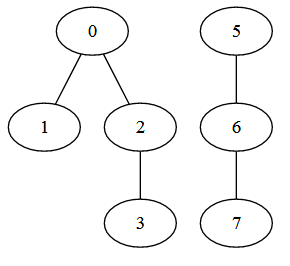
\includegraphics[width=\textwidth]{imgs/graph.PNG}
    \caption{Graphe original, non orienté}
  \end{minipage}
  \hfill
  \begin{minipage}[b]{0.4\textwidth}
    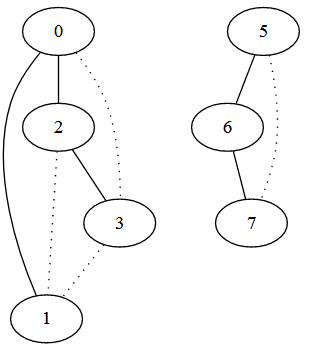
\includegraphics[width=\textwidth]{imgs/graphFT.PNG}
    \caption{Graphe et sa fermeture transitive}
  \end{minipage}
\end{figure}

\iffalse
Code du graphe (enlever les dotted pour le graphe original)

graph G {
	0 -- 1
    0 -- 2
    2 -- 3
    5 -- 6
    6 -- 7
    3 -- 1 [style=dotted]
    5 -- 7 [style=dotted]
    2 -- 1 [style=dotted]
    0 -- 3 [style=dotted]
}
\fi

On va attribuer à chaque chemin une valeur de confiance ou score de confiance qui va déterminer si ce chemin peut être utilisé pour évaluer un fait. Ce score va d'abord dépendre du degré (liens avec d'autres entités) des noeuds traversés. Une entité générique aura un degré important ce qui diminuera le score de confiance, ex : un pays, une grande organisation, etc. D'un autre côté ce score sera plus élevé s'il traverse des noeuds moins génériques, ex : personne, livre, etc. En effet un lien entre deux entités sera plus pertinent si le chemin ne traverse que des entités avec peu de relations et le contexte sémantique sera plus précis. En suivant la même logique lorsque deux entités sont directement liées, on va leur accorder un score de confiance maximal : il n'y a pas d'intermédiaires.

Le chemin qui aura le score le plus élevé sera le chemin le plus court et qui traversera les entités les moins générique. C'est ce que l'on va appeler la proximité sémantique. Cette proximité sémantique représente le sens qui relie deux entités. Pour un fait donné, est-ce que c'est deux entités mise bout à bout ont du sens ? 

Pour le moment nous avons vu comment choisir un chemin entre deux entités, qui va nous permettre ensuite de déterminer si un fait est vrai ou faux. 
\\*
Pour illustrer ceci, prenons un exemple, soit des faits qui lient des villes avec des pays. Pour chaque pays et chaque villes on va tester l'assertion : \enquote{La capitale du pays x est y}.

\begin{figure}[h]
\centering
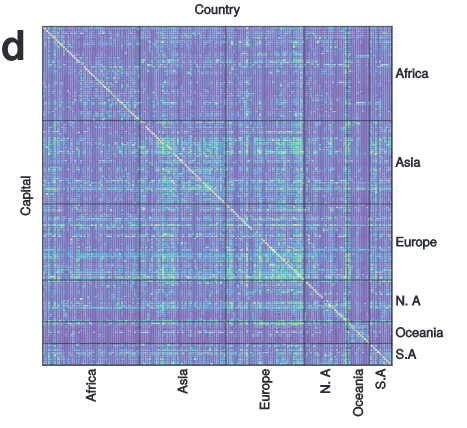
\includegraphics[draft=false, scale=0.5]{imgs/country_cap_check.PNG}
\caption{Pays et capitales groupées par continent}
\label{fig1}
\end{figure}

\todo{\url{http://www.kurzweilai.net/a-computational-algorithm-for-fact-checking}}

Plus un point est clair et plus le fait a de chance d'être vrai. Le chemin entre un pays et sa capitale possède une proximité sémantique plus forte que le chemin entre un pays et n'importe quelle autre ville. Bien que cette méthode soit très basique, elle apporte des résultats satisfaisant. Le taux de réussite selon les datasets utilisés varie entre 61\% et 95\%. Cet exemple prouve que le fact checking peut se faire au travers de graphes de connaissances. 

\paragraph{Critique} Cette méthode permet de faire du fact checking sur des faits simples. Elle se fait entre deux entités clairement définies. Le champs des possibles pour les faits à vérifier est donc limité.

Problème de scalabilité, important d'avoir le verdict instantanément.

Nous verrons plus tard, avec des méthodes plus avancées, certains problèmes inhérents à l'utilisation de KG pour le fact checking.

Ciampaglia et al. [8] propose
an approach that relies on a single short, specific path to
differentiate a true fact from a false one. Although intuitive,
their algorithm fails to account for the semantics of the target
predicate

\todo{Ouvrir sur la seconde approche knowledge stream et montrer qu'il améliore cette approche}

\todo{A lire : https://searchengineland.com/google-researchers-introduce-system-rank-web-pages-facts-not-links-215835}